\documentclass[
    iai, % Saisir le nom de l'institut rattaché
    en, % Saisir le nom de l'orientation
    % confidential, % Décommentez si le travail est confidentiel
]{heig-tb}

\usepackage[nooldvoltagedirection,european,americaninductors]{circuitikz}

\signature{mbernasconi.svg} % Remplacer par votre propre signature vectorielle.

\makenomenclature
\makenoidxglossaries
\makeindex

\addbibresource{bibliography.bib}

\input{nomenclature}
\input{acronyms}
\input{glossary}
% Auteur du document (étudiant-e) en projet de Bachelor
\author{Maël Michod}

% Activer l'option pour l'accord du féminin dans le texte
\genre{female}

% Titre de votre travail de Bachelor
\title{Modèle \LaTeX~de rapport de Bachelor}

% Le sous titre est optionnel
\subtitle{Travail de Bachelor}

% Nom du professeur responsable
\teacher {Prof. Y. Chevallier (HEIG-VD)}

% Mettre à jour avec la date de rendu du travail
\date{\today}

% Numéro de TB
\thesis{7212}



\surroundwithmdframed{minted}

%% Début du document
\begin{document}
\selectlanguage{french}
\maketitle
\frontmatter
\clearemptydoublepage

%% Requis par les dispositions générales des travaux de Bachelor
\preamble
\authentification

%% Résumé / Résumé publiable / Version abrégée
\begin{abstract}
    \input{abstract}
\end{abstract}

%% Sommaire et tables
\clearemptydoublepage
{
    \tableofcontents
    \let\cleardoublepage\clearpage
    \listoffigures
    \let\cleardoublepage\clearpage
    \listoftables
    \let\cleardoublepage\clearpage
    \listoflistings
}

\printnomenclature
\clearemptydoublepage
\pagenumbering{arabic}

%% Contenu
\mainmatter
\chapter{Introduction}
\input{introduction.tex}
\input{examples.tex}

\chapter{État de l'art}

\section{Normes de qualité de l'énergie pour les réseaux publics de distribution MT/BT}

\subsection{EN50160}

La norme EN50160 \cite{en50160} décrit les limites ou les valeurs caractéristiques de la tensions attendues livrées aux divers bornes d'un réseau public de distribution.

"Le présent document spécifie, aux bornes de livraison de l'utilisateur du réseau, les caractéristiques principales de tension fournies par un réseau public d'électricité en courant alternatif basse tension, moyenne tension, haute tension et très haute tension dans des conditions normales d'exploitation."

"Les réseaux industriels sont exclus du domaine d'application de l'EN 50160."

"Le présent document a pour objet de définir et de décrire les valeurs caractérisant la tension d'alimentation fournie telles que: la fréquence, l'amplitude, la forme d'onde et la symétrie des tensions entre phases."

"En exploitation normale, ces caractéristiques sont sujettes à des variations dues à des modifications de charge du réseau, des perturbations émises par certains équipements et par l'apparition de défauts principalement dus à des causes externes.

Les caractéristiques varient de façon aléatoire, à la fois dans le temps à des bornes de livraison données, et dans l'espace, à un instant donné. A cause de ces variations, les valeurs des caractéristiques indiquées dans le présent document peuvent être dépassées en un petit nombre d'occasions."





\subsubsection{Caractéristiques de l'alimentation basse tension}

"Le présent article décrit les caractéristiques de tension de l'électricité fournie par les réseaux basse tension publics. Une distinction est faite ci-après entre:

— les phénomènes continus, c'est-à-dire des écarts par rapport à la valeur nominale se produisant de manière continue dans le temps. De tels phénomènes se produisent principalement à cause du type de charge ou de production, des variations de la charge ou des charges non linéaires;

— les événements de tension, c'est-à-dire des écarts brusques et significatifs par rapport à la forme d'onde normale ou souhaitée. Les événements de tension sont généralement dus à des événements imprévisibles (par exemple des défauts) ou des causes extérieures (comme les conditions climatiques, les actions de tiers);

— d'autres phénomènes, c'est-à-dire des phénomènes se produisant en présence de systèmes de communication par le réseau d'alimentation électrique (MCS) et/ou d'équipements utilisant une technologie de commutation raccordés au réseau."





\subsubsection{Tension harmonique}

"Dans les conditions normales d'exploitation, pendant chaque période d'une semaine, 95 \% des valeurs efficaces de chaque tension harmonique individuelle sur 10 min doivent être inférieures ou égales aux valeurs indiquées dans le Tableau 1. Des tensions plus élevées pour un harmonique donné peuvent être dues à des résonances.
De plus, le taux global de distorsion harmonique de la tension fournie (incluant tous les harmoniques jusqu'au rang 40) doit être inférieur ou égal à 8 \%."

\begin{figure}[H]
    \begin{center}
        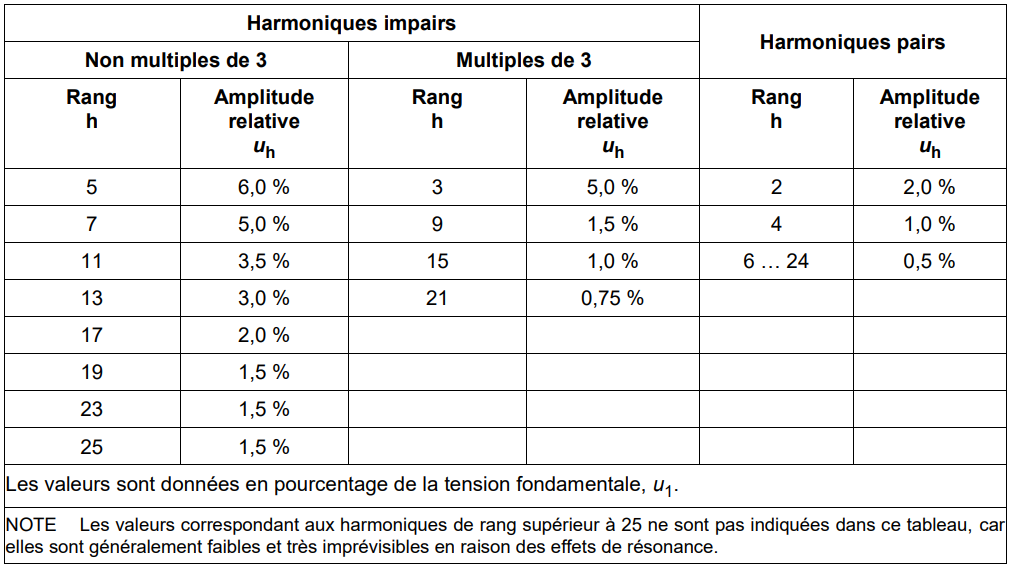
\includegraphics[width=\textwidth]{assets/figures/tab_en50160.png}
    \end{center}
    \caption{Valeurs des tensions harmoniques individuelles aux bornes de livraison BT}
    \label{tab_en50160}
\end{figure}

Comme le souligne la note en bas de tableau, les harmoniques de rang supérieur à 25 ne sont pas indiqués.





\subsubsection{Tension interharmonique}

"Le niveau des interharmoniques est en augmentation en raison du nombre croissant de convertisseurs de fréquence et autres équipements similaires de contrôle-commande. Les niveaux d'interharmoniques restent à l'étude et seront fournis dans un futur amendement.
Dans certains cas, les interharmoniques, même de faible niveau, provoquent du papillotement ou des interférences avec les systèmes de télécommande centralisée."




\subsection{IECTR61000-3-14}


\subsubsection{Domaine d'application}
"La présente partie de l'IEC 61000, qui est informative par nature, fournit des recommandations sur les principes qui peuvent être utilisés pour déterminer les exigences relatives au raccordement des installations perturbatrices aux réseaux publics d'alimentation à basse tension (BT)."

"Le présent rapport traite de la répartition de la capacité du réseau à absorber les perturbations. Il n'explique pas comment atténuer les perturbations ni comment l'aptitude du réseau peut être augmentée."

"Le présent rapport technique s'applique uniquement aux installations raccordées aux réseaux publics d'alimentation BT qui alimentent ou peuvent alimenter d'autres charges ou installations BT. Il est présumé s'appliquer aux grandes installations dont les dimensions dépassent une taille minimale. Cette taille minimale (Smin) doit être spécifiée par le gestionnaire ou le propriétaire du réseau en fonction des caractéristiques du réseau."


Le présent rapport technique traite divers perturbations conduites à basse fréquence, notament les harmoniques et les interharmoniques, qui sont émises par les installations BT.

"Etant donné que les lignes directrices décrites dans le présent rapport reposent nécessairement sur certaines hypothèses de simplification, il n'est pas assuré que cette approche constitue toujours la solution optimale pour toutes les situations. Il convient d'utiliser l'approche recommandée en faisant preuve de souplesse et de discernement en ce qui concerne l'ingénierie, lors de l'application de toute ou partie des procédures d'évaluation indiquées."


"Le présent rapport fournit les procédures recommandées pour définir les limites d'émission dans le cas des grandes installations BT."



\subsubsection{Niveau de compatibilité}

"Il s'agit de valeurs de référence pour la coordination des émissions et de l'immunité des appareils connectés à ou alimentés par un réseau d'alimentation afin d'assurer la CEM sur l'ensemble du réseau (y compris le système et les appareils connectés)."

"Il est admis que le gestionnaire du réseau ne puisse pas contrôler continuellement tous les points d'un réseau. C'est pourquoi il convient d'évaluer les niveaux de compatibilité à l'échelle du réseau, mais aucune méthode d'évaluation n'est actuellement fournie pour l'évaluation à un emplacement spécifique."

\paragraph{Harmoniques :}

"Les niveaux de compatibilité spécifiés dans l'IEC 61000-2-2 pour les tensions harmoniques sur les réseaux BT doivent être étudiés par rapport aux états quasi stationnaires ou en régime établi. Ils sont donnés en tant que valeurs de référence pour les effets à long terme et pour les effets à très court terme.

– Les effets à long terme concernent principalement les conséquences thermiques sur les câbles, transformateurs, moteurs, condensateurs, etc. Ils proviennent de niveaux d'harmoniques maintenus pendant 10 min ou plus.

– Les effets à très court terme concernent principalement les perturbations agissant sur des dispositifs électroniques qui peuvent être sensibles à des niveaux d'harmoniques maintenus pendant 3 s ou moins. Les transitoires ne sont pas compris dans ces effets.

Le Tableau 1 donne les niveaux de compatibilité relatifs aux composantes harmoniques de la tension pour les effets à long terme. Le niveau de compatibilité correspondant à la distorsion harmonique totale est THD = 8 \%."

\begin{figure}[H]
    \begin{center}
        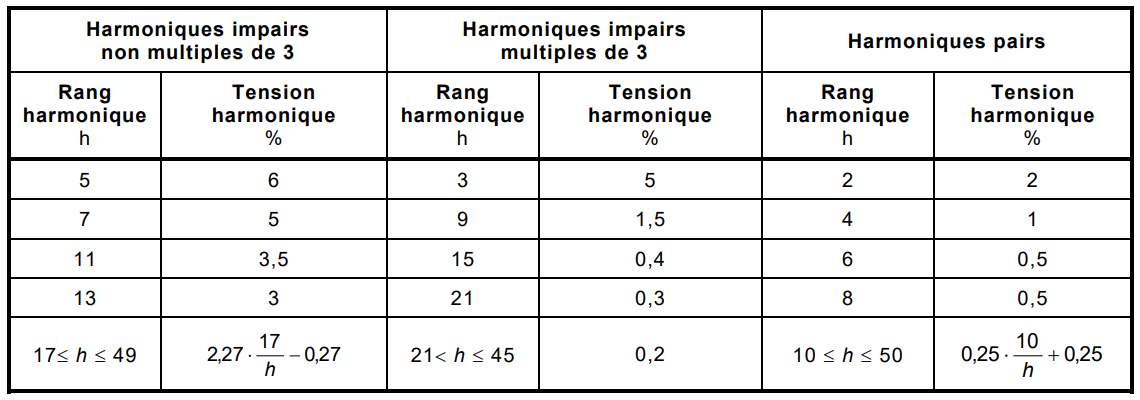
\includegraphics[width=\textwidth]{assets/figures/IECTR61000_tab1.png}
    \end{center}
    \caption{Niveaux de compatibilité pour les tensions harmoniques sur les réseaux BT (pourcentages de la composante fondamentale) issus de l'IEC 61000-2-2}
    \label{IECTR61000_tab1}
\end{figure}

"En ce qui concerne les effets à très court terme (voir l'IEC 61000-2-2), les niveaux de compatibilité relatifs aux composantes harmoniques de la tension sont égaux aux valeurs indiquées dans le Tableau 1, multipliées par un coefficient khvs, où khvs est calculé comme suit:"

\begin{equation}
    k_{hvs} = 1.3 + \frac{0.7}{45} \cdot (h-5)
\end{equation}

"En référence aux effets à très court terme des harmoniques, le niveau de compatibilité pour la distorsion harmonique totale est THD = 11 \%."



\paragraph{Interharmoniques :}

"L'état des connaissances concernant les perturbations électromagnétiques impliquées dans les tensions interharmoniques est toujours en cours de développement."

"La norme IEC 61000-2-2 ne donne des niveaux de compatibilité que dans le cas de tensions interharmoniques à une fréquence proche de la fréquence fondamentale (50 Hz ou 60 Hz), ce qui donne lieu à une modulation de l'amplitude de la tension d'alimentation et engendre un phénomène de papillotement. Le niveau de compatibilité pour une tension interharmonique dans ce cas est fondé sur un niveau de papillotement de Pst = 1 (voir la Figure 2 de l'IEC 61000-2-2)."


\subsubsection{Niveaux de plannification}

\paragraph{Valeurs indicatives des niveaux de planification :}

"Il s'agit de niveaux qui peuvent être utilisés à des fins de planification pour évaluer l'incidence sur le réseau d'alimentation de toutes les installations perturbatrices. Les niveaux de planification sont spécifiés par le gestionnaire ou le propriétaire du réseau pour tous les niveaux de tension du réseau et peuvent être considérés comme des objectifs de qualité internes du gestionnaire ou du propriétaire du réseau."

"Les niveaux de planification sont définis au cas par cas, selon la structure et les caractéristiques du réseau, et aucune valeur précise ne peut être donnée."


\paragraph{Procédure d'évaluation par rapport aux niveaux de plannification :}

"Les méthodes de mesure à utiliser sont les méthodes de mesure de classe A définies dans l'IEC 61000-4-30. Il convient de retirer de l'évaluation les données marquées conformément à la norme. Pour plus de clarté, lorsque des données sont marquées, le percentile utilisé pour calculer les indices définis ci-dessous est calculé à l'aide des données (non marquées) valables uniquement."

"Pour chaque type de perturbation, la période de mesure minimale correspond à une semaine d'activité commerciale normale. Il convient que la période de surveillance comprenne une partie de la période, où sont attendus les niveaux de perturbation maximaux."

"Un ou plusieurs des indices suivants peuvent être utilisés pour comparer les niveaux de perturbation réels aux niveaux de planification."

"Pour les tensions harmoniques, les indices suivants sont utilisés:

– il convient que la valeur hebdomadaire de 95 \% de Uh,sh (valeur efficace des composantes harmoniques sur des périodes "courtes" de 10 min) ne dépasse pas le niveau de planification;

– il convient que la valeur quotidienne la plus élevée de probabilité de 99 \% de Uh,vs (valeur efficace des composantes harmoniques sur des périodes "très courtes" de 3 s) ne dépasse pas le niveau de planification multiplié par le facteur de multiplication khvs donné par l'Equation (1) vis-à-vis des effets à très court terme des harmoniques."



\subsubsection{Illustration des concepts de CEM}

"Dans un réseau d'alimentation complet, il est inévitable qu'un certain niveau d'interférence se produise à certaines occasions, d'où le risque de superposition entre les distributions des niveaux de perturbation et des niveaux d'immunité (voir la Figure 1). Les niveaux de planification sont généralement inférieurs ou égaux au niveau de compatibilité; ils sont spécifiés par le gestionnaire ou le propriétaire du réseau. Les niveaux d'essai d'immunité sont spécifiés par les normes pertinentes ou sont fixés par accord entre les fabricants et les clients."

\begin{figure}[H]
    \begin{center}
        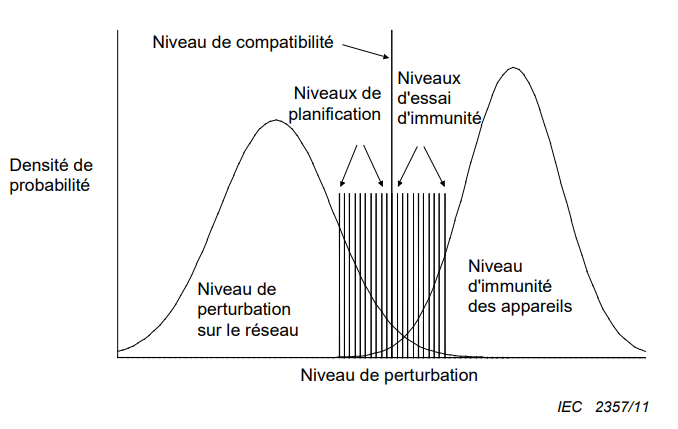
\includegraphics[width=\textwidth]{assets/figures/IECTR61000_tab2.png}
    \end{center}
    \caption{Représentation des concepts de base de la qualité de la tension, avec statistiques de durée/emplacement couvrant l'ensemble du réseau}
    \label{IECTR61000_tab2}
\end{figure}


\begin{figure}[H]
    \begin{center}
        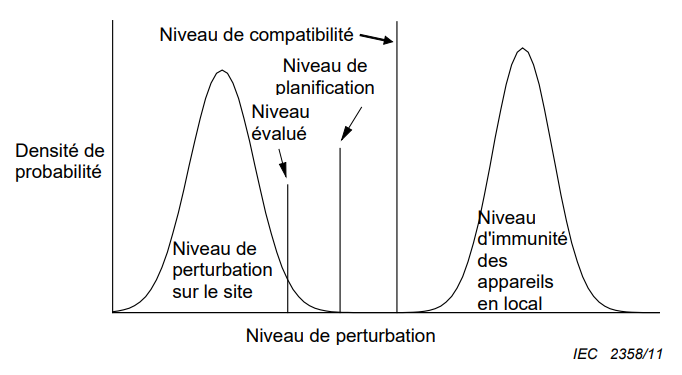
\includegraphics[width=\textwidth]{assets/figures/IECTR61000_tab3.png}
    \end{center}
    \caption{Représentation des concepts de base de la qualité de la tension, avec statistiques temporelles pertinentes pour un site du réseau}
    \label{IECTR61000_tab3}
\end{figure}

"Comme le montre la Figure 2, les distributions de probabilité des niveaux de perturbation et d'immunité sur un site sont normalement plus restreintes que pour l'ensemble du réseau d'alimentation; sur la plupart des emplacements, il y a peu voire aucun chevauchement des distributions des niveaux de perturbation et d'immunité. Les interférences ne constituent donc généralement pas une préoccupation majeure, et les appareils sont présumés fonctionner de manière satisfaisante. La compatibilité électromagnétique est donc plus probable que semble le suggérer la Figure 1."


\subsubsection{Niveaux d'émission}

"L'approche de coordination recommandée dans le présent rapport repose sur les différents niveaux d'émission déterminés à partir des niveaux de planification. Pour cette raison, les mêmes indices sont appliqués à la fois lors de l'évaluation des mesures réelles par rapport aux limites d'émission et aux niveaux de planification.
Un ou plusieurs des indices suivants peuvent être utilisés pour comparer le niveau d'émission réel à la limite d'émission du client."

"Pour les émissions d'harmoniques, les indices suivants sont utilisés:

– il convient que la valeur hebdomadaire de 95 \% de Uh,sh (ou Ih,sh), la valeur efficace des composantes harmoniques sur des périodes "courtes" de 10 min, ne dépasse pas la limite d'émission EUhi (ou EIhi);

– il convient que la valeur quotidienne la plus élevée de probabilité de 99 \% de Uh,vs (ou Ih,vs), la valeur efficace des composantes harmoniques sur des périodes "très courtes" de 3 s, ne dépasse pas la limite d'émission multipliée par le facteur khvs donné par l'Equation 1."


\subsubsection{Point d'évaluation}

"Le point d'évaluation (POE) est le point où sont évalués les niveaux d'émission de l'installation d'un client donné afin de vérifier la conformité aux limites d'émission. Il s'agit également du point sur le réseau d'alimentation considéré, au niveau duquel sont définis les niveaux de planification. Ce point peut être le point de connexion (POC), le point de couplage commun (PCC) de l'installation perturbatrice."

\subsubsection{Concept du niveau d'émission}

"Le niveau d'émission d'une installation dans le réseau d'alimentation représente l'amplitude du vecteur de tension perturbatrice (ou de courant perturbateur) causé par l'installation considérée au point d'évaluation. En cas d'harmoniques ou de déséquilibre, le concept général peut être représenté à la Figure 3 par le vecteur Udi et sa contribution (ainsi que le vecteur de perturbation Ud0 causé par toutes les autres sources de perturbations lorsque l'installation considérée n'est pas raccordée au réseau) au vecteur de perturbation Ud mesuré au point d'évaluation, lorsque l'installation a été raccordée."

\begin{figure}[H]
    \begin{center}
        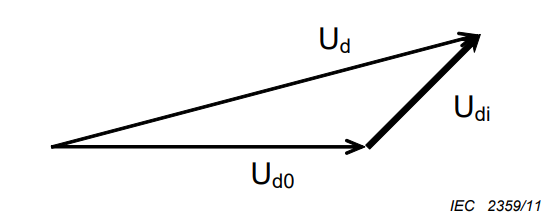
\includegraphics[width=\textwidth]{assets/figures/IECTR61000_fig1.png}
    \end{center}
    \caption{Représentation du vecteur d'émission Udi et de sa contribution au vecteur de perturbation Ud mesuré au point d'évaluation}
    \label{IECTR61000_fig1}
\end{figure}

"Lorsque le vecteur d'émission entraîne une augmentation des niveaux de perturbation sur le réseau (c'est-à-dire |Ud| > |Ud0|), il est nécessaire que le niveau d'émission défini ci-dessus (c'est-à-dire |Udi|) soit inférieur aux limites d'émission évaluées conformément aux articles pertinents du présent rapport.

Pour les harmoniques, l'interaction entre le réseau d'alimentation et l'installation du client peut dans certains cas entraîner une amplification ou une réduction du niveau de distorsion de tension à un rang harmonique donné (c'est-à-dire en raison de la création d'une condition de résonance parallèle ou en série, ou d'un effet d'annulation). Une amplification est possible même lorsque l'installation elle-même ne génère pas d'harmoniques de ce rang. Etant donné que le présent rapport traite des exigences de coordination CEM, de telles situations d'amplification sont prises en compte avec cette définition des niveaux d'émission réels."


\subsubsection{Caractéristiques de l'impédance du réseau}

"Pour les harmoniques, la procédure décrite dans le présent rapport ne prend pas en compte tous les cas de résonances sur le réseau BT. Lorsque des résonances peuvent se produire, une évaluation ou une simulation approfondie est nécessaire. Il importe de noter que les installations des autres clients ont également une incidence sur l'impédance du réseau. Les batteries de condensateurs qui peuvent modifier les résonances ou créer d'autres résonances (voir Robert et al.) doivent faire l'objet d'une attention particulière."


\subsubsection{Loi de sommation générale}

"La coordination des perturbations conduites exige l'adoption d'hypothèses pertinentes pour la sommation des perturbations produites par différentes installations perturbatrices. Dans le cas de perturbations de type harmonique, fluctuation ou déséquilibre dues à des charges perturbatrices aléatoires, le niveau de perturbation global réel en tout point d'un réseau de distribution est le résultat de la sommation vectorielle de chaque source de perturbation.

A partir de l'expérience acquise, une loi de sommation générale peut être adoptée pour application au niveau d'un réseau d'alimentation:"

\begin{equation}
    D = \sqrt[\alpha]{\sum_i D_i^\alpha}
\end{equation}

où:
D est l'amplitude du niveau de perturbation obtenu pour l'agrégation considérée des sources;
Di est l'amplitude du niveau de perturbation produit par l'une des sources de perturbations à agréger;
$\alpha$ est un exposant qui dépend principalement de 3 facteurs:
- le type de perturbation;
- la valeur choisie pour la probabilité que la valeur réelle ne dépasse pas la valeur calculée;
- le degré de variation aléatoire des perturbations par rapport à l'amplitude et à la phase.


"NOTE 1 Cette loi de sommation générale est une approximation statistique de la sommation vectorielle sous-jacente pour de nombreuses sources aléatoires. Elle est spécifiquement utilisée pour l'allocation des limites d'émission aux installations afin de définir une augmentation raisonnable du niveau de perturbation qui peut être tolérée par le gestionnaire ou le propriétaire du réseau.

NOTE 2 Dans le cas d'une source spécifique de perturbation, il demeure évident que la sommation vectorielle peut, dans la pratique, entraîner une réduction du niveau de perturbation, même si la loi de sommation générale ne peut donner qu'une augmentation."

"Pour les besoins du présent rapport, l'ensemble d'exposants indiqué dans le Tableau 3 peut être utilisé en l'absence d'autres informations spécifiques."
\begin{figure}[H]
    \begin{center}
        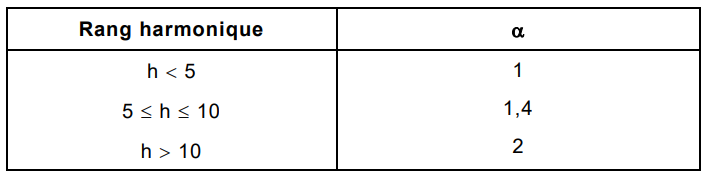
\includegraphics[width=\textwidth]{assets/figures/IECTR61000_tab4.png}
    \end{center}
    \caption{Exposant de sommation pour les harmoniques (valeurs indicatives)}
    \label{IECTR61000_tab4}
\end{figure}

\subsubsection{Principes généralisés - Limites d'émission d'harmoniques pour les installations déformantes sur les réseaux BT}

\paragraph{Étape 1 - Evaluation simplifiée des émissions perturbatrices :}

"Pour les petites installations, comme les maisons résidentielles, le gestionnaire ou le propriétaire du réseau peut généralement s'appuyer sur les limites d'émission d'harmoniques pour que les appareils respectent les niveaux de planification. Par exemple, l'IEC 61000-3-2 et l'IEC 61000-3-12 sont des normes de familles de produits qui définissent les limites d'émission d'harmoniques pour les appareils raccordés aux réseaux publics d'alimentation BT.

Une installation peut être raccordée au réseau d'alimentation sans examen supplémentaire si tous les appareils de l'installation satisfont aux limites d'émission pertinentes définies dans l'IEC 61000-3-2 et l'IEC 61000-3-12, et si la condition suivante est remplie:"
\begin{equation}
    S_i < S_{min}
\end{equation}

où:
- Si est la puissance souscrite pour l'installation (i) du client;
- Smin est la valeur minimale de la puissance souscrite pour les installations BT à laquelle s'applique la procédure de définition des limites d'émission fournie dans le présent rapport.

"La valeur minimale de la puissance souscrite pour les installations BT (Smin) dans le cadre du présent rapport doit être spécifiée par le gestionnaire ou le propriétaire du réseau en fonction des caractéristiques du réseau."

"Au contraire, pour les grandes installations (Si ≥ Smin) ou si certains appareils de l'installation ne respectent pas les limites d'émission correspondantes définies dans l'IEC 61000-3-2 et l'IEC 61000-3-12, il convient que le gestionnaire ou le propriétaire du réseau veille davantage à ce que les niveaux de planification ne soient pas dépassés.

Dans ce cas, le raccordement d'une installation déformante peut être toléré à l'étape 1 si les trois conditions suivantes sont remplies:

a. le client n'utilise pas de condensateurs d'amélioration du facteur de puissance (PFC, Power Factor Correction) et/ou de filtres harmoniques;

b. le rapport suivant est vérifié:
\begin{equation}
    \frac{S_i}{S_{sc}} \leqslant 1\%
\end{equation}

c. pour chaque rang harmonique, les émissions de courants harmoniques sont inférieures aux limites prudentes définies par le gestionnaire ou le propriétaire du réseau à partir des caractéristiques du réseau:
\begin{equation}
    \frac{I_{hi}}{S_i} \leqslant E_{lh}
\end{equation}

où:
- Si est la puissance apparente souscrite pour l'installation (i) du client;
- Ssc est la puissance de court-circuit au point d'évaluation;
- Ihi est le courant harmonique de rang h produit par l'installation déformante (i);
- Ii est le courant efficace (fréquence fondamentale) correspondant à la puissance souscrite pour l'installation (i) du client (Si / UN√3, où UN est la tension nominale entre phases du réseau BT);
- EIh est la limite d'émission de courants harmoniques de rang h définie par le gestionnaire ou le propriétaire du réseau à partir des caractéristiques prudentes du réseau pour l'évaluation des installations à l'étape 1.



\paragraph{Étape 2 - Limites d'émission par rapport aux caractéristiques réelles du réseau :}

"Compte tenu de la capacité d'absorption réelle du réseau, en raison du facteur de transfert entre le réseau MT amont et le réseau BT considéré et des différences de phase des courants harmoniques ainsi que de l'impédance du réseau et des charges futures, des émissions supérieures à celles définies selon les critères de l'étape 1 peuvent être accordées."

"Ainsi, la méthode suggérée dans le présent rapport pour les grandes installations BT prend en compte les émissions de courants par les différents appareils. Il est admis ici par hypothèse que les limites de courant des appareils ont été définies de manière à ce que, si le réseau BT est utilisé à sa pleine capacité par ces appareils, les niveaux globaux de perturbation de tension ne dépassent pas les niveaux de planification. De ce fait, la procédure suivante a pour objet de fixer les limites d'émission de courants pour les grandes installations BT de l'étape 2:

- dans un premier temps, la contribution globale admissible de l'ensemble des grandes et petites installations raccordées à un réseau BT donné au niveau global de perturbation de tension sur ce réseau BT est déterminée;

- la contribution d'une grande installation BT est établie de telle sorte que le niveau global de perturbation de tension sur le réseau BT soit inférieur ou égal au niveau obtenu lorsque cette grande installation est remplacée par un groupe de petites installations de puissance totale identique.

Ainsi, le niveau de perturbation dû aux émissions de toutes les sources d'harmoniques raccordées au réseau ne dépasse pas le niveau de planification."


"L'objectif est de définir les limites d'émission de courants harmoniques pour les grandes installations BT (voir l'Article 1). Dans un premier temps, il est nécessaire de déterminer la contribution globale acceptable du réseau BT considéré aux distorsions de tension.

Dans un premier temps, il est nécessaire d'appliquer la loi de sommation générale (Equation 3) pour déterminer la contribution globale acceptable maximale de l'ensemble des sources d'harmoniques présentes sur un réseau BT particulier. En effet, pour chaque rang harmonique, la tension harmonique réelle sur un réseau BT résulte de la combinaison vectorielle de la tension harmonique émise par le réseau MT amont et de la tension harmonique émise par l'ensemble des sources déformantes raccordées au réseau BT considéré. Il convient que cette tension harmonique totale ne dépasse pas le niveau de planification du réseau BT. Ainsi, le niveau global de tension harmonique qui peut être alloué à l'ensemble des installations raccordées au réseau BT considéré est donné par (pour plus d'informations, voir l'Article C.3):"

\begin{equation}
    G_{hBT} = \sqrt[\alpha]{L_{hBT}^\alpha - (T_{hMT} \cdot L_{hMT})^\alpha}
\end{equation}

où:
– GhLV est la contribution globale acceptable maximale de l'ensemble des installations BT qui peuvent être alimentées par le réseau considéré, à la he tension harmonique en tout point du réseau BT (exprimée en pourcentage de la tension fondamentale);
– LhLV est le niveau de planification pour le he harmonique sur le réseau BT;
– LhMV est le niveau de planification pour le he harmonique sur le réseau MT amont;
– ThML est le coefficient de transfert des distorsions de la tension harmonique entre le réseau MT amont et le réseau BT considéré dans le rang harmonique h (si nécessaire, il peut être déterminé par simulation ou par mesurage);
– $\alpha$ est l'exposant de la loi de sommation (Tableau 3).

"NOTE Pour des raisons de simplicité, le facteur de transfert utilisé dans cette équation est considéré comme une valeur unique pour chaque rang harmonique.

Pour une évaluation simplifiée, les coefficients de transfert ThML du réseau MT sur un réseau BT peuvent être pris comme égaux à 1. Dans la pratique, toutefois, il peut être inférieur à 1 pour les ordres harmoniques élevés, en raison de l'effet d'amortissement des charges BT, ou supérieur à 1 (généralement entre 1 et 3) en condition de faible charge, si des résonances sont présentes. Il est de la responsabilité du gestionnaire ou du propriétaire du réseau de déterminer les valeurs pertinentes en fonction des caractéristiques du réseau."


Limite d'émission individuelle :

\begin{equation}
    G_{hBT} = K_{hBT} \cdot G_{hMT}
\end{equation}

où:
- GhB est la contribution globale acceptable de l'ensemble des installations BT qui peuvent être alimentées par le réseau considéré, à la he tension harmonique sur le jeu de barres du poste BT (exprimée en pourcentage de la tension fondamentale);
- KhB est le facteur de réduction au rang harmonique h, qui correspond au rapport du niveau de tension harmonique sur le jeu de barres BT induit par l'ensemble des installations raccordées au réseau BT considéré au niveau maximal de la tension harmonique sur le réseau BT induit par ces installations (ce niveau maximal est généralement atteint à l'extrémité de l'un des départs d'alimentation). Ce facteur de réduction ne dépend pas des niveaux d'émission d'harmoniques, mais uniquement de la structure du réseau BT (nombre et longueur des départs d'alimentation, distribution des installations des clients, etc.) et de l'exposant α utilisé pour la loi de sommation. Des informations sur la détermination de KhB en fonction des caractéristiques du réseau BT sont fournies à l'Annexe D: un tableau simplifié donne quelques exemples de valeurs types de KhB pour les réseaux BT.


"Compte tenu des considérations ci-dessus et de celles de l'Annexe C, les limites d'émission d'harmoniques pour une grande installation BT (i) exprimées par rapport au courant sont données par:"
\begin{equation}
    E_{lhi} = \frac{U_N^2}{S_i} \cdot G_{hBT} \cdot \sqrt[\alpha]{\frac{S_i}{S_t}} \cdot min(\frac{K_{hBT}}{Z_{hBT}};\frac{1}{Z_{hi}})
\end{equation}

où:
- EIhi est la limite d'émission de courants harmoniques de rang h pour l'installation (i) raccordée à un réseau BT (\%: exprimée en pourcentage du courant de l'installation correspondant à sa puissance souscrite, Si / UN√3);
- UN est la tension nominale entre phases du réseau BT (V);
- GhLV est la contribution globale acceptable maximale de l'ensemble des installations BT qui peuvent être alimentées par le réseau considéré, à la he tension harmonique en tout point du réseau BT (\%:exprimée en pourcentage de la tension fondamentale);
- Si est la puissance apparente souscrite pour l'installation (i) du client (VA);
- St est la capacité d'alimentation totale du réseau BT considéré, avec la possibilité d'augmenter la charge ultérieurement. St peut également inclure la contribution de la production décentralisée (VA);
- $\alpha$ est l'exposant de la loi de sommation (Tableau 3);
- min (x, y) représente la valeur minimale de x et de y;
- KhB est le facteur de réduction au rang harmonique h, déterminé à l'aide de l'Equation (8);
- ZhB est le module de l'impédance harmonique du réseau sur le jeu de barres du poste BT (Ω);
- Zhi est le module de l'impédance harmonique du réseau au point d'évaluation de l'installation (i) (Ω).

"Les limites d'émission d'harmoniques données par l'Equation (9) dépendent des facteurs de réduction KhB. Dans certains réseaux BT, les valeurs types de KhB peuvent donner des limites harmoniques trop souples. Dans ces cas, il convient de déterminer les valeurs de KhB à partir des caractéristiques réelles du réseau BT. L'Annexe D décrit une méthode pour estimer KhB. L'approche ci-dessus ne prend pas en compte les résonances sur le réseau BT. Lorsque des résonances peuvent se produire, des méthodes avancées éventuellement associées à des simulations sont nécessaires pour l'étape 3."

\paragraph{Etape 3 - Validation des niveaux d'émission supérieurs sous conditions}

"Les considérations générales fournies en 4.3 s'appliquent à l'étape 3 pour les harmoniques.

Une méthode générale qui peut s'appliquer à l'étape 3 est également décrite à l'Annexe E."

\paragraph{Limites d'émission pour les interharmoniques :}

"Les tensions interharmoniques peuvent être additionnées de manière arithmétique seulement si les fréquences et les phases sont égales. Ces conditions sont rarement remplies et pendant de courtes périodes. C'est pourquoi, dans la pratique, la valeur de la tension interharmonique la plus élevée peut ne pas être supérieure au double.

Si la tension interharmonique d'une grande installation BT est inférieure à 0,1 \%, aucune perturbation n'est prise en compte."




\subsubsection{Diagrammes récapitulatifs de la procédure d'évaluation}

\begin{figure}[H]
    \begin{center}
        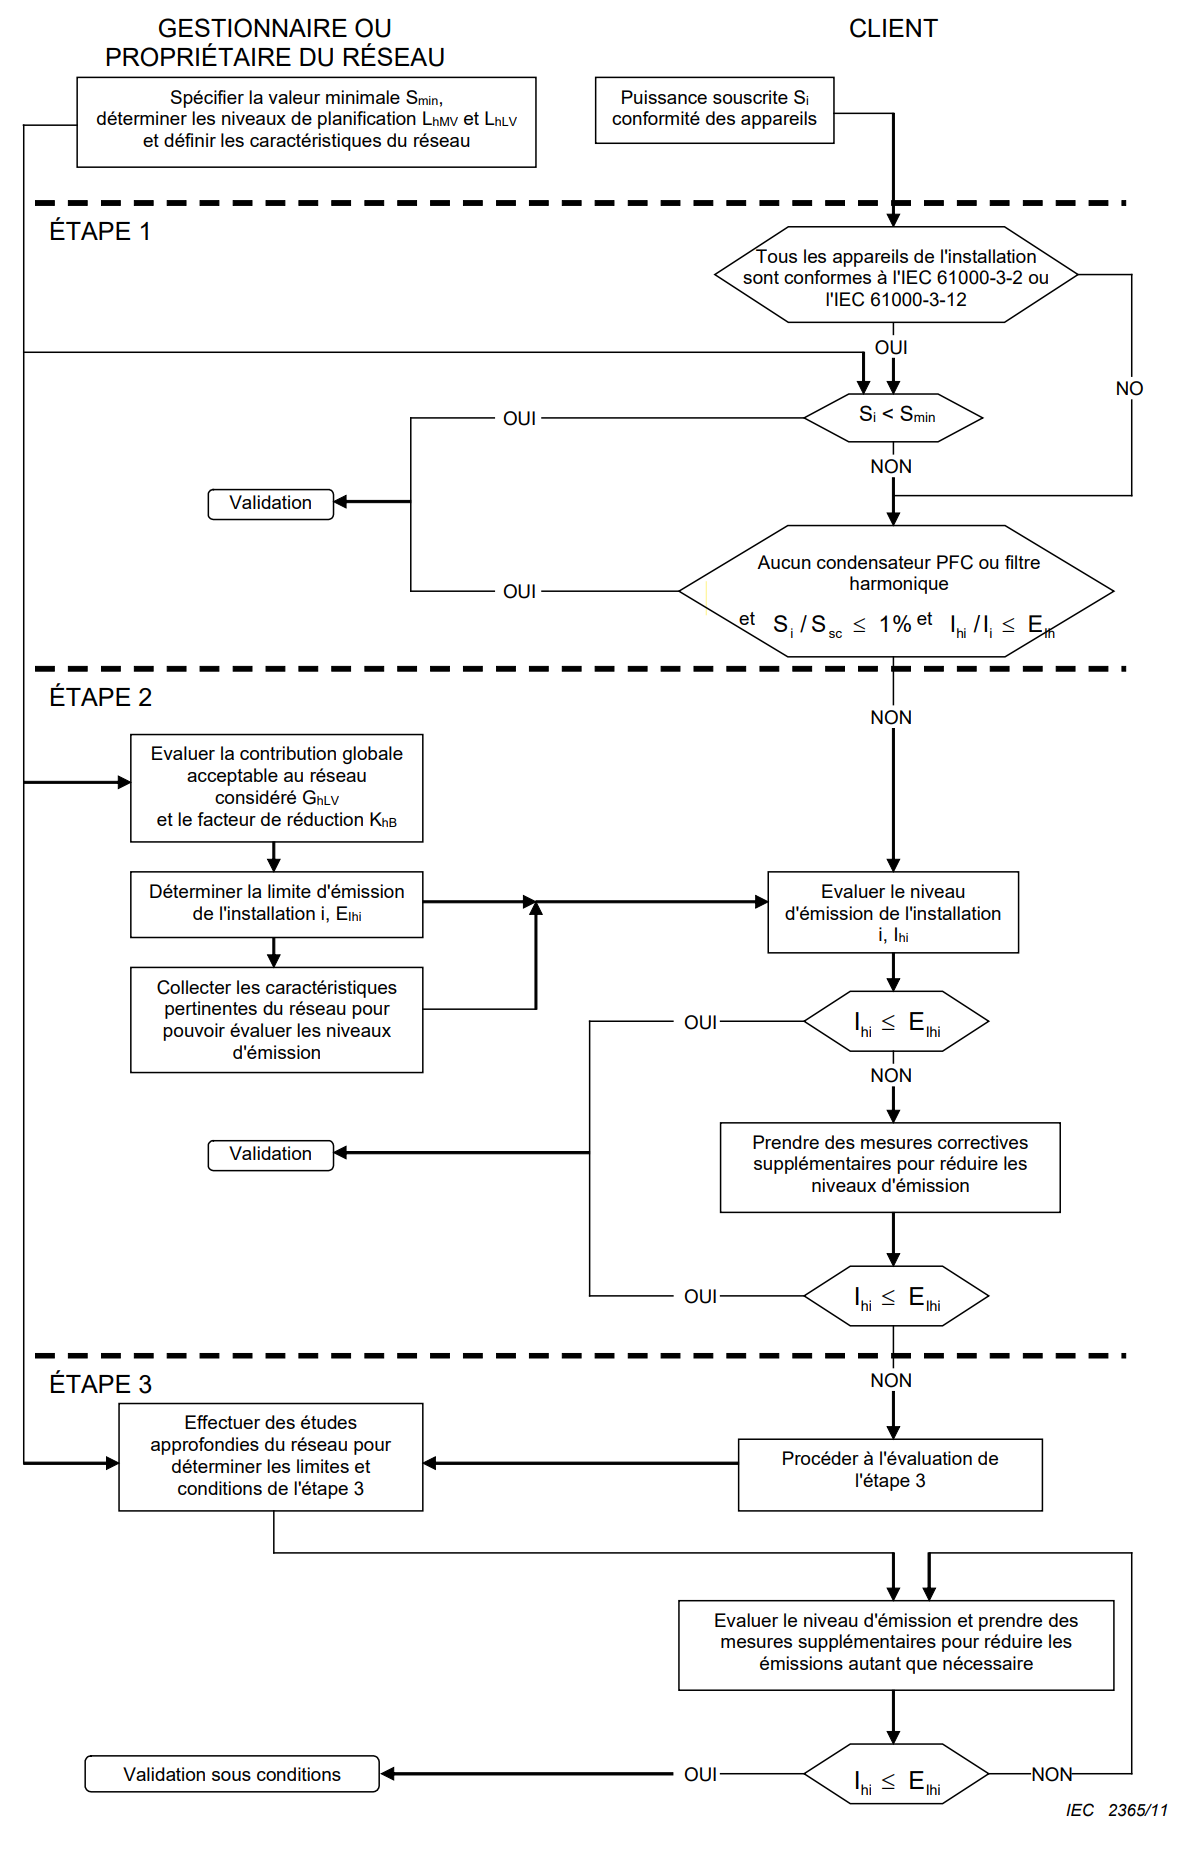
\includegraphics[width=\textwidth]{assets/figures/IECTR61000_sch.png}
    \end{center}
    \caption{Diagramme de la procédure d'évaluation pour les harmoniques}
    \label{IECTR61000_sch}
\end{figure}









\section{Excédent d'harmoniques et problèmes de dysfonctionnement liés aux onduleurs BT}



\section{Systèmes de mesure de la qualité de l'énergie au niveau du réseau et des onduleurs}



\section{Technologies des compteurs intelligents}



\section{Étude sur l'agrégation théorique des harmoniques en simulation}



\section{Méthode Machin Learning}

\chapter{Conclusion}
\input{conclusion.tex}

\clearpage
\printbibliography

\appendix
\appendixpage
\addappheadtotoc

%%if
\chapter{Première annexe}

Les annexes n'ont pas un contenu \underline{normatif} mais \underline{descriptif}. Tout contenu annexé ne doit pas être nécessaire à la bonne compréhension du travail.

Les annexes contiennent généralement :

\begin{itemize}
    \item les dessins mécaniques (mises en plan);
    \item les schémas électriques détaillés;
    \item des photographies du projet;
    \item des scripts et des extraits de code source;
    \item des documents techniques \pex \emph{datasheet};
    \item des développements mathématiques.
\end{itemize}
\section{Sous section}
\lipsum[1]
%%fi

\let\cleardoublepage\clearpage
\backmatter

\label{glossaire}
\printnoidxglossary
\label{index}
\printindex

% Le colophon est le dernier élément d'un document qui contient des notes de l'auteur concernant la mise en page et l'édition du document : il est parfaitement optionnel.
\input{colophon.tex}

\end{document}
